\documentclass[11pt]{article}
\usepackage{aahomework}
\usepackage{mathtools}
\usepackage{subcaption}
\usepackage{epstopdf}
\usepackage{float}
%\tikzstyle{blk}=[circle,inner sep=0pt,minimum size =4pt,draw,fill=black,line width=0.8pt]
%\tikzstyle{blanknode}=[circle,inner sep=3pt,minimum size =8pt,draw,line width=0.8pt]
%\tikzstyle{blk}=[circle,inner sep=0pt,minimum size =4pt,draw,fill=black,line width=0.8pt]
%
%\geometry{letterpaper, textwidth=17cm, textheight=22cm}

%\usetikzlibrary{arrows}
%\usetikzlibrary{plotmarks}

\title{Lecture 1}
\author{A. Agarwal}
\date{December 7, 2012}

\newcommand{\keyphrase}{\textbf}

\begin{document}
%\maketitle

\section*{System of Linear Equations}

A \keyphrase{system of linear equations} is a set of equations, all of which are linear (powers of $x$ and $y$ are at most $1$).
\begin{align*}
\left\{\begin{aligned}
3x &= 1
\\
x + 2y &= 3
\end{aligned}
\right.
\end{align*}

There are two ways of interpreting such as system:
\begin{enumerate}
\item{
\textbf{Geometric way}
}
\item{
\textbf{Algebraic way}
}
\end{enumerate}

As an example, consider what does $x=1$ represent? Some may say a \keyphrase{point}, others may say a \keyphrase{line}.

It is important to consider the \keyphrase{ambient space} in which the equation(s) are to be considered.

Examples of the object $x=1$ in the ambient spaces $\bbR, \bbR^2,$ and $\bbR^3$.

Consider again the system
\begin{align}
\left\{\begin{aligned}
3x &= 1
\\
x + 2y &= 3
\end{aligned}
\right.
\label{eq:system1}
\end{align}
Since there are two variables, we know that the system is in at least two dimensions (maybe more). For now, let us consider the system in two dimensions. What will be the solution?

\vspace{.5cm}

The equation $3x=1$ represents a line, as does $x+2y=3$. Figure [x] shows these lines:

Line $3x=1$

Line $x+2y=3$

Once we have this geometric picture of the system, a solution to the system will be a point common to both lines.

This is a geometric picture of the system. We still need some sort of algebraic way of finding the exact solution. In this case, the first equation gives us that $x = 1/3$, and the second equation gives us that
\begin{align*}
y
= \frac{3-x}{2}
= \frac{3 - \frac{1}{3}}{2}
= \frac{8}{6}
= \frac{4}{3}
\end{align*}

We now have the coordinates of the solution to the equations: $(1/3, 4/3)$. Formally, we can now claim that we have found the solution $(1/3, 4/3)$ to the system \eqref{eq:system1} considered in $\bbR^2$.

\vspace{1cm}

In the above example, there is only one solution. We may ask ourselves, given any system, will there always be one solution, can there be more than one solution, or may there not be any solution? It turns out that examining these possibilities through a geometric perspective holds the answer and will allow us to generalize the answer to this question.


Two lines may either intersect at one point (Figure \ref{fig:lineintersections}a), yielding a \keyphrase{unique solution}; never intersect (Figure \ref{fig:lineintersections}b), which results in \keyphrase{no solutions} existing; or be on top of one another (Figure \ref{fig:lineintersections}c), which results in \keyphrase{infinitely many solutions}.

One unique solution.

No solution.

Infinitely many solutions.

The ways in which two lines may or may not intersect.

A natural question is whether it is possible for there to be finitely many solutions, and more than one solution? Geometrically, we can see that since two points define a line, two lines cannot intersect at more than one point without being the same line. The situation in $\bbR^2$ seems to be then that we can have either one solution, no solutions, or infinitely many solutions.

It is natural to ask whether we can generalize this to higher dimensions. Let us consider $\bbR^3$.

\begin{align*}
\left.
\begin{aligned}
x - y + z &= 1
\\
2x - 3y + 7z &= 2
\end{aligned}
\right\}
\end{align*}

In $\bbR^3$, these equations represent \keyphrase{planes}. If we are given two planes, they may intersect, and if they do, they must intersect in a line, similar to how pages in a book intersect at the spine of the book. In this case, there are infinitely many solutions. Alternatively the planes may not intersect at all, in which case there are no solutions. The planes may also be on top of one another; that is, they are the same plane, in which case there are also infinitely many solutions.

\begin{figure}[H]
\centering
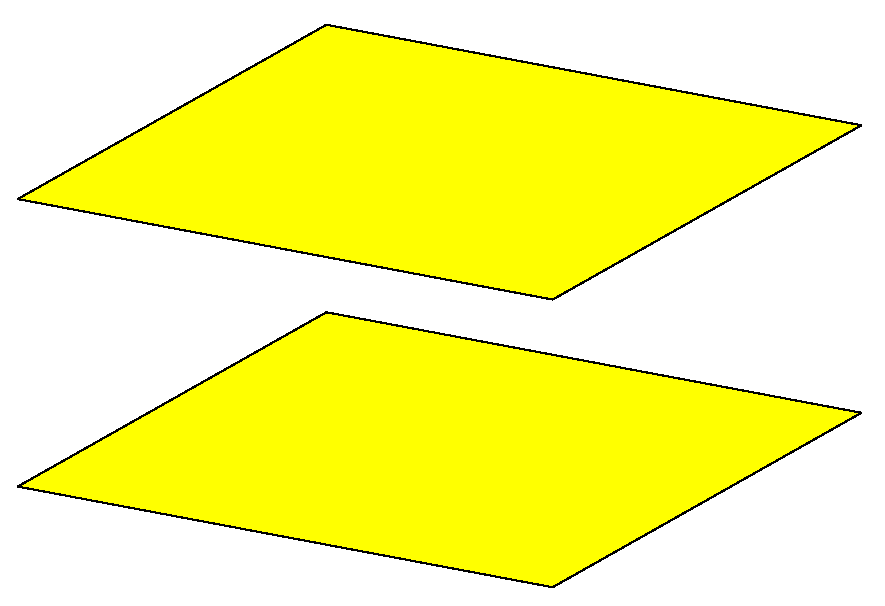
\includegraphics[width=7cm]{parallelplanes.eps}
\hspace{.5cm}
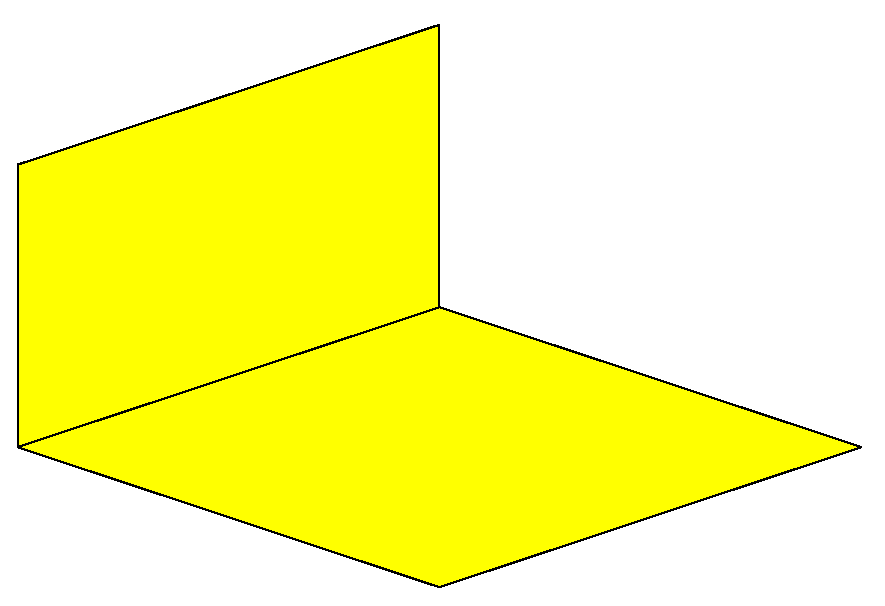
\includegraphics[width=7cm]{intersectingplanes.eps}
\caption{Parallel and intersecting planes.}
\end{figure}

Can it be that two planes may have a unique solution? It seems to be that the answer is no. But if we are given a third plane, we may have a unique solution. Consider for instance the corner of a room. Here the floor and two walls are meeting at a unique point.

\begin{align*}
\left.
\begin{aligned}
3x - y + z &= 7
\\
x - y + z &= 1
\\
2x - 3y + 7z &= 2
\end{aligned}
\right\}
\qquad
\text{A system consisting of three planes}
\end{align*}


This tells us that in $\bbR^2$ or $\bbR^3$, there seem to be always either one solution, no solutions, or infinitely many solutions. In fact, we will find that it is always that case that:


The number of solutions in $\bbR^n$ of a system of linear equations will be only one of
\begin{enumerate}
\item{
One solution
}
\item{
Zero solutions
}
\item{
Infinitely many solutions
}
\end{enumerate}

Right now we cannot conclude this. Later we will, but that proof comes from understanding these systems in more algebraic terms.

\newpage

\section*{Solve system of linear equations}

Before we move on to solving systems of linear equations, it is important to note that the variables used in these equations are not the focus of the problem. Consider the following two systems:
\begin{align*}
\left.
\begin{aligned}
x - 2y &= 3
\\
2x + 3y &= 7
\end{aligned}
\right\}
&&
\left.
\begin{aligned}
a - 2b &= 3
\\
2a + 3b &= 7
\end{aligned}
\right\}
\end{align*}
The equations in the two systems are identical except for the variables, so in fact they represent the same system.

The important part of these systems are the coefficients of the variables. What we will do is put the coefficients in a matrix:
\begin{align*}
\left[ \begin{matrix}
1 & -2 & 3
\\
2 & 3 & 7
\end{matrix} \right]
\end{align*}
In order to preserve the fact that the $3$ and $7$ are on the right-hand-side of the equations, we will put a vertical bar within the matrix:
\begin{align*}
\left[ \begin{matrix}
1 & -2 & 3
\\
2 & 3 & 7
\end{matrix} \right]
\end{align*}
This is referred to as an \keyphrase{augmented matrix}. 

\begin{align*}
\left[
\begin{matrix}
A & \vec{b}
\end{matrix}
\right]
&=\left[ \begin{matrix}
1 & -2 & 3
\\
2 & 3 & 7
\end{matrix} \right]
\end{align*}

In general, we say the left part $A$ of the augmented matrix is the \keyphrase{coefficient matrix}, and the right part $\vec{b}$ is the \keyphrase{right-hand-side vector}, or the constant vector.

Every system of linear equations can be translated into an augmented matrix, and every augmented matrix can be translated back into a system of linear equations.

This notation saves time and we will be using it a lot.


\begin{center}
\begin{minipage}[t]{.48\linewidth}
\subsection*{Row Picture}
\begin{align*}
\left.
\begin{aligned}
x - 2y &= 3
\\
2x + 3y &= 7
\end{aligned}
\right\}
\begin{aligned}
\longleftarrow
\\
\longleftarrow
\end{aligned}
\quad\text{Rows}
\end{align*}
Row Picture: Intersection of two lines
\end{minipage}
\begin{minipage}[t]{.48\linewidth}
\subsection*{Column Picture}
\begin{align*}
x
\begin{bmatrix}
1
\\
2
\end{bmatrix}
+
y
\begin{bmatrix}
-2
\\
3
\end{bmatrix}
=
x
\begin{bmatrix}
3
\\
7
\end{bmatrix}
\end{align*}
Column Picture: Can $\begin{bmatrix}3\\7\end{bmatrix}$ be written as a linear combination of $\begin{bmatrix}1\\2\end{bmatrix}$ and $\begin{bmatrix}-2\\3\end{bmatrix}$?
\end{minipage}
\end{center}

The advantages of the column picture may not be apparent now, but looking at things in the language in linear combinations will be very useful later.

It is important to note that in the above case, the row and column picture are in the same number of dimensions. Consider instead

\begin{align*}
\left.
\begin{aligned}
x - y + z &= 21
\\
3x + y - 3z &= 0
\end{aligned}
\right\}
&&
\begin{aligned}
x \begin{bmatrix}1\\3\end{bmatrix}
+
y \begin{bmatrix} -1\\1\end{bmatrix}
+
z \begin{bmatrix} 1\\-3\end{bmatrix}
&=
\begin{bmatrix}21\\0\end{bmatrix}
\end{aligned}
\end{align*}

Here the row picture is the intersection of two planes in $\bbR^3$. The column picture is a linear combination of vectors in $\bbR^2$.

These perspectives will be useful, and in particular pay attention to the idea of linear combinations.

\subsection*{Solving a system}
Consider the system in $\bbR^2$,
\begin{align*}
\left.
\begin{aligned}
x &= 1
\\
y &= 3
\end{aligned}
\right\}
\qquad
\longrightarrow
\qquad
\left.
\begin{matrix}
x & + & 0y & = 1
\\
0x & + & y & = 3
\end{matrix}
\right\}
\end{align*}
We can easily convert the system to and from an augmented matrix:
\begin{align*}
\left[
\begin{matrix}
1 & 0 & 1
\\
0 & 1 & 3
\end{matrix}
\right]
\end{align*}
This is in a sense our `Dream augmented matrix', in that from it we can directly determine the solution to the system. The technical term for this sort of matrix is a \keyphrase{row-reduced echelon form matrix}.

In some sense then, the row-reduced echelon form matrix is our goal when solving systems of linear equations. The question is, how will we go from a general matrix to a row-reduced echelon form matrix? To do so, we will learn \keyphrase{row operations} 

\end{document}
